\documentclass[a4paper,11pt]{book}

\usepackage[T1]{fontenc}
\usepackage[utf8]{inputenc}
\usepackage[LGR,T1]{fontenc} % notice LGRx instead of LGR
\usepackage{lmodern}
\usepackage[final]{pdfpages} 
\usepackage[top=2cm, bottom=3cm, outer=3cm, inner=4cm, headsep=14pt]{geometry}
\usepackage{textgreek}
\usepackage{csquotes}
\usepackage[french]{babel}
\usepackage{fancyhdr}
\usepackage{xsim}
\usepackage{tasks}
\usepackage[absolute]{textpos}
\usepackage{ascii}
\usepackage{eurosym}
\usepackage{amsthm}
\usepackage{circuitikz}
\usepackage{url}


\theoremstyle{definition}
\newtheorem{exmp}{Example}[section]

\bibliographystyle{abbrv}
\pagestyle{fancy}
\fancyhf{}
\renewcommand{\footrulewidth}{1pt}
\renewcommand{\thesection}{\arabic{section}}

\lhead{Architecture des ordinateurs}
\rhead{Implémentation des portes logiques}
\rfoot{Page \thepage}

\begin{document}

\chapter{Implémentation des portes logiques}
Dans ce chapitre, nous allons proposer quelques solutions pour créer des portes logiques avec différents types de transistors. Loin de donner un catalogue exhaustif, ni même complet, des implémentations possibles, l'objectif de ce chapitre est de décrire des éléments de base et de donner au lecteur des pistes qui lui permettront d'approfondir le sujet le cas échéant.

Nous supposons ici que le lecteur sait déjà ce qu'est une porte logique, une table de vérité et quelle table de vérité correspond aux portes logiques de base.

\section{Transistors bipolaires}
Nous allons commencer par une série de portes réalisées avec des transistors bipolaires. Ce n'est pas ce qui est le plus fréquemment utilisé dans les circuits intégrés, mais les schémas relativement simples permettent une excellente introduction du sujet.

\subsection{Porte NON (NOT ou inverseur)}
Pour obtenir une porte NON, nous utilisons un seul transistor qui agit comme interrupteur commandé : figure \ref{fig:NOT}.

Dans ce circuit, lorsque la tension $V_A$ vaut 0, il n'y a pas de courant qui circule dans la base ($I_B$ vaut 0), le transistor est donc fermé ($R_T = \infty)$. La tension en sortie vaut alors $Vcc$ ($R_1$ agit en \emph{pull up}).

À l'inverse, si A vaut $Vcc$, on a alors une chute de tension entre la base et l'émetteur du transistor de $0.7V$, donc sur $R2$ une chute de tension de $Vcc - 0.7V$ et un courant de base\footnote{Loi d'Ohm: $U=RI$ ou $I = \frac{U}{R}$} :
\[I_B = \frac{Vcc - 0.7}{R_2}\]

On peut calculer le courant entre le collecteur et l'émetteur $I_{CE} = \beta \times I_B$. La chute de tension sur la résistance $R_1$ se calcule aussi avec loi d'Ohm : $U_{R_1} = R_1 \times (\beta \times I_B)$, soit : 

\[U_{R_1} = \beta \times R_1 \times \frac{Vcc - 0.7}{R_2}  \]

En posant :

\[ \frac{\beta R_1}{R_2} >> 1\]

On voit que $U_{R_1}$ tendra rapidement vers $Vcc$.

Donc nous aurons en sortie une tension de $Vcc - U_{R_1} \approx 0$.

On peut "interpréter" ces calculs de la manière suivante : avec une tension Vcc appliquée à la base, un courant passe entre la base et l'émetteur, ce qui "ouvre" le transistor. Le transistor ouvert, la chute de tension se fait uniquement sur la résistance $R_1$ et donc la sortie est à zéro.

\begin{figure}
\centering
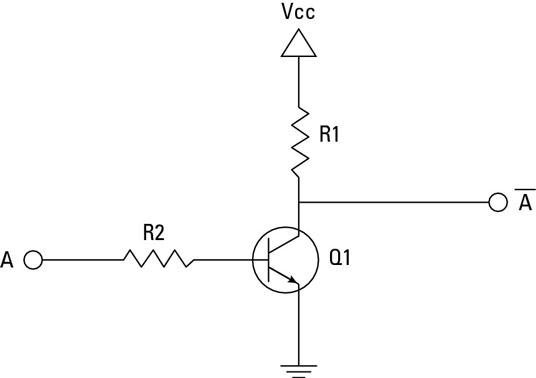
\includegraphics[width=0.5\textwidth]{media/ImplementationGates/311277.image0.jpg}
\caption{Porte NON (inverseur)}
\label{fig:NOT}
\end{figure}

\subsection{Porte OU}

La figure \ref{fig:OR} nous propose une porte OU. Si les deux entrées sont à 0, alors les deux transistors sont \emph{fermés}, et la sortie est reliée à la terre. Si un ou les deux transistors sont ouverts, alors la chute de tension sur le ou les transistors est de 0.7V et la chute de tension sur la résistance \emph{pull down} de $4.7k\Omega$ est de quasi $Vcc$, la sortie est donc à 1.

\begin{figure}
\centering
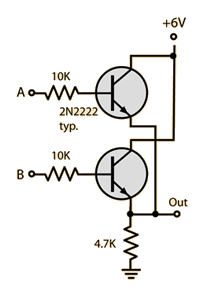
\includegraphics[width=0.5\textwidth]{media/ImplementationGates/or4.png}
\caption{Porte OU }
\label{fig:OR}
\end{figure}

\subsection{Porte ET}

En appliquant les mêmes raisonnements, on voit sur le schéma à la figure \ref{fig:AND} qu'il faut cette fois que les deux transistors soient ouverts pour que la tension en sortie passe de 0 à $Vcc$.

\begin{figure}
\centering
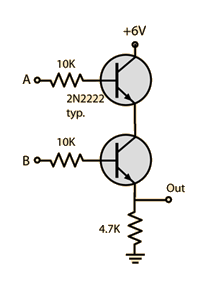
\includegraphics[width=0.5\textwidth]{media/ImplementationGates/and4.png}
\caption{Porte ET}
\label{fig:AND}
\end{figure}

\subsection{Porte OU exclusif}
Pour la porte XOR, le circuit est un peu plus compliqué. On y parviendra en combinant des portes logiques ET et OU selon la relation: 

\[ A \oplus B = \bar{A}B + A\bar{B} \]

Et donc une combinaison de portes.

\section{Transistors MOSFET}
Il est assez simple de concevoir des portes logiques avec des transistors FET au niveau des couches de Silicium et des dopages à mettre en place. On parle de circuit CMOS lorsque ce dernier intègre des transistors MOSFET de type canal P et/ou N.

\subsection{Porte NON (inverseur)}
Une porte NON s'obtient très facilement avec deux transistors MOSFET de type N et P respectivement, comme nous le voyons sur la figure \ref{fig:NOT_MOS}.

\begin{figure}
\centering
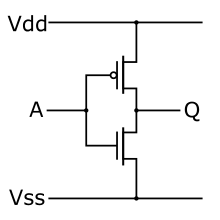
\includegraphics[width=0.5\textwidth]{media/ImplementationGates/220px-CMOS_Inverter.svg.png}
\caption{Porte NON (inverseur) (Source : Wikimedia)}
\label{fig:NOT_MOS}
\end{figure}

\subsection{Porte ET}
Dans la figure \ref{fig:ET_MOS}, nous trouvons une implémentation d'une porte ET et sa réalisation avec des masques correspondant aux différentes couches de silicium et de dépôts métalliques dans la figure \ref{fig:ET_CMOS_MASK}.

\begin{figure}
\centering
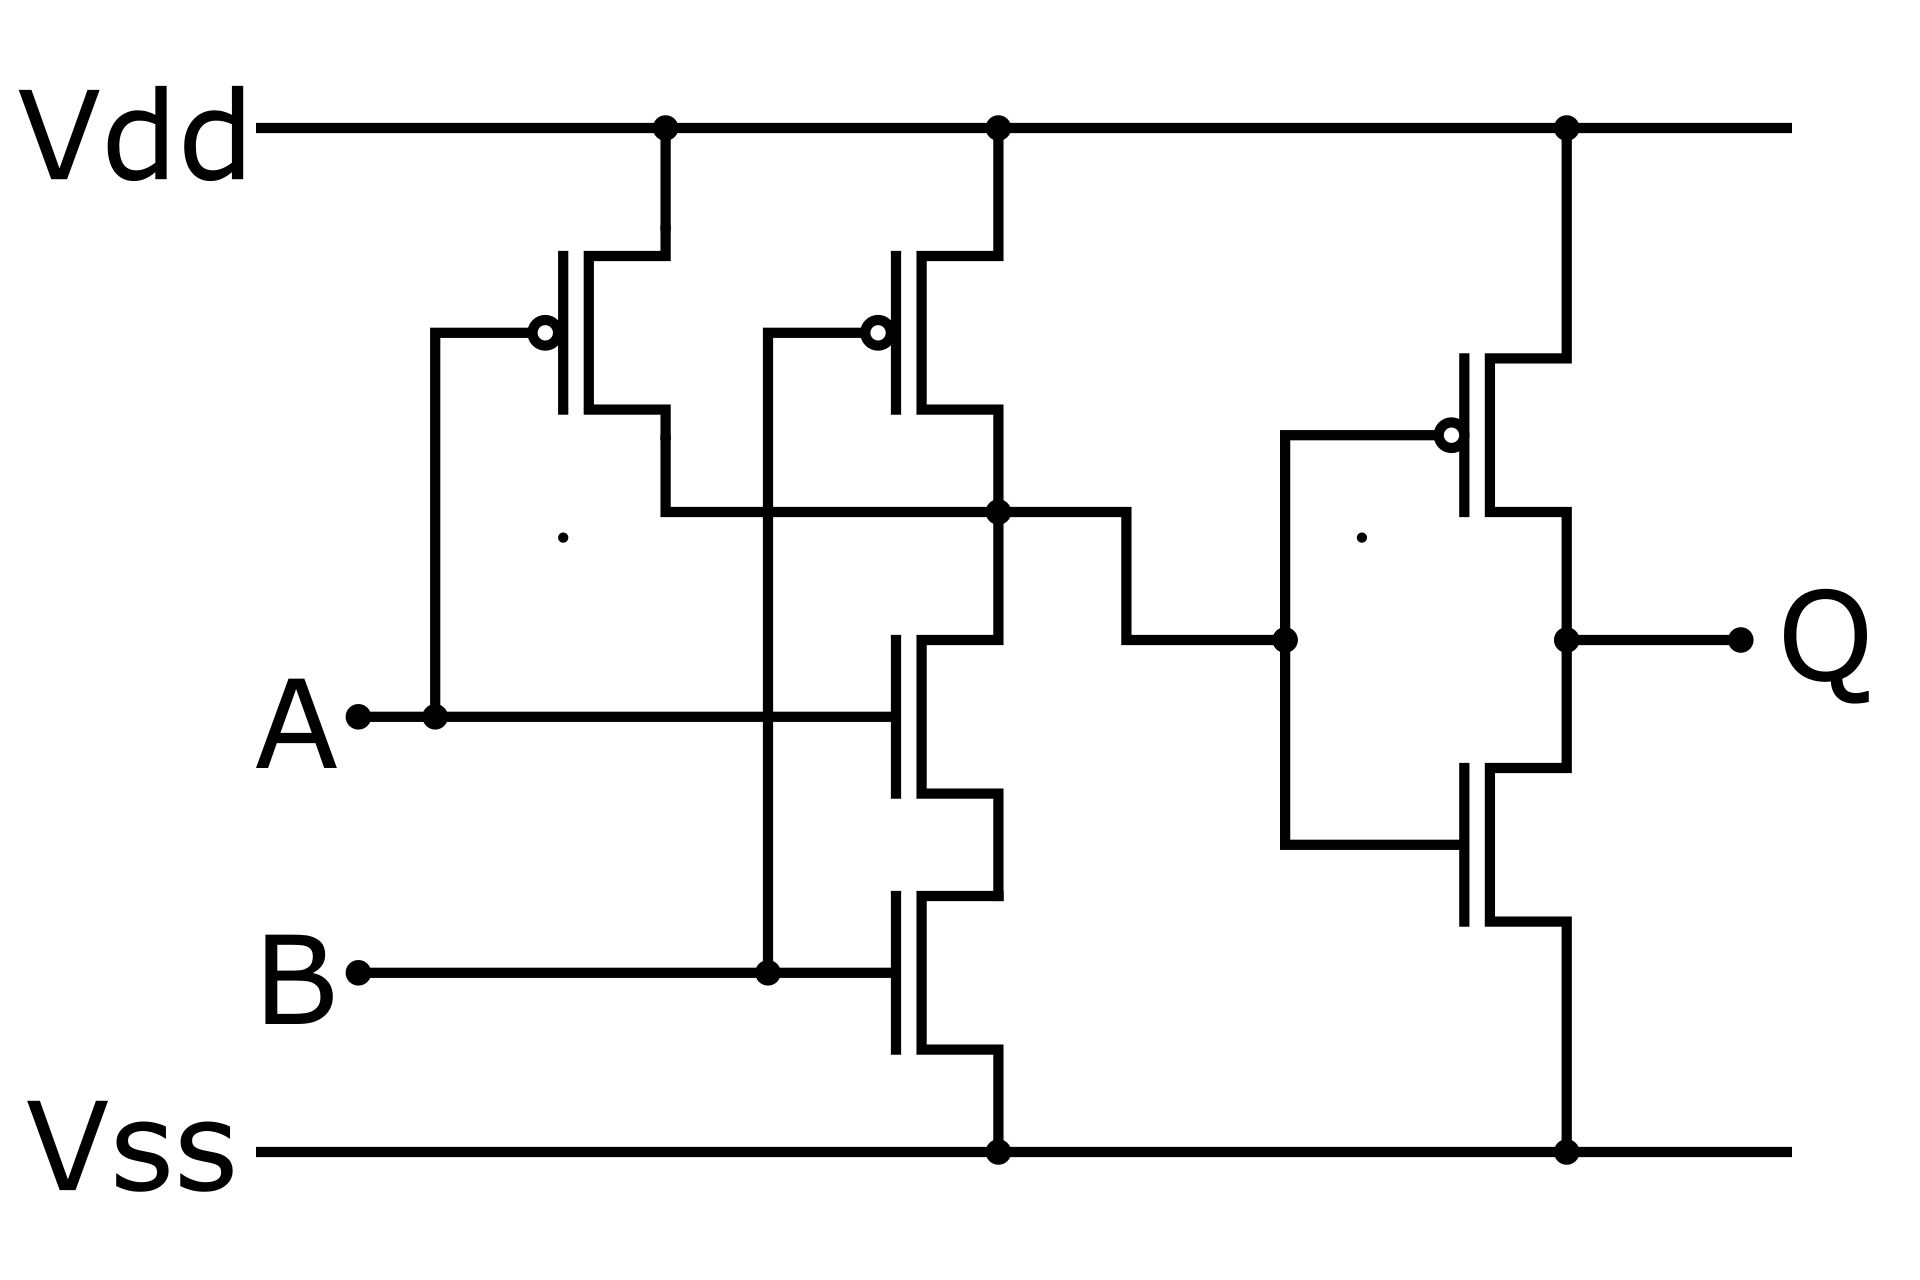
\includegraphics[width=0.5\textwidth]{media/ImplementationGates/CMOS_AND_Layout.svg.png}
\caption{Porte ET avec des transistors MOSFET (Source : Wikimedia)}
\label{fig:ET_MOS}
\end{figure}

\begin{figure}
\centering
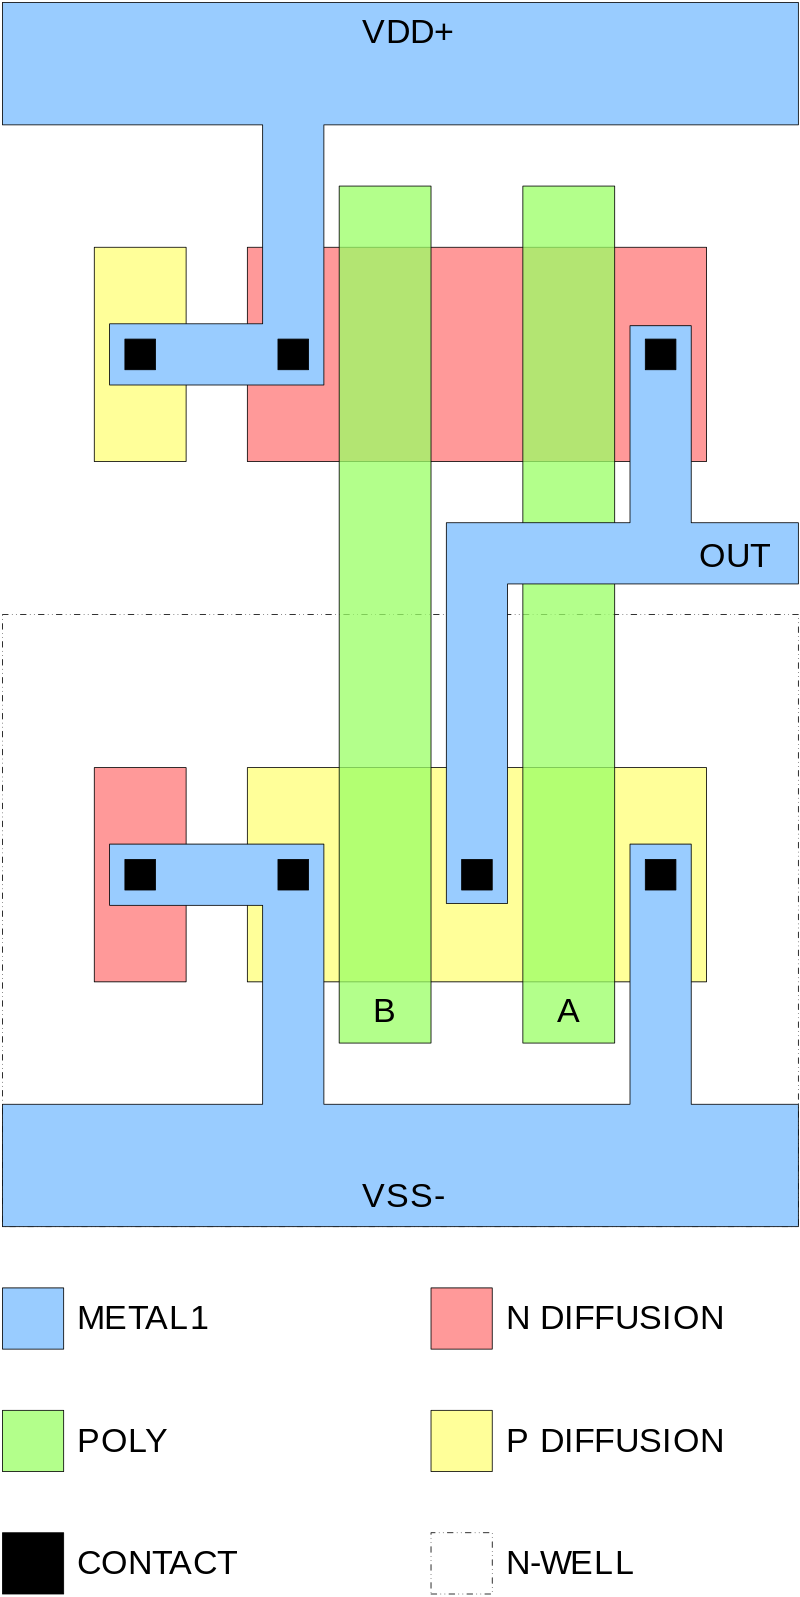
\includegraphics[width=0.5\textwidth]{media/ImplementationGates/800px-CMOS_AND_Silicon.svg.png}
\caption{Masques du circuit CMOS ET (Source : Wikimedia)}
\label{fig:ET_CMOS_MASK}
\end{figure}


\subsection{Porte NON-ET}
Dans la figure \ref{fig:NON-ET_MOS}, nous trouvons une implémentation d'une porte NON-ET et sa réalisation avec des masques correspondant aux différentes couches de silicium et de dépôts métalliques dans la figure \ref{fig:NON-ET_CMOS_MASK}.

\begin{figure}
\centering
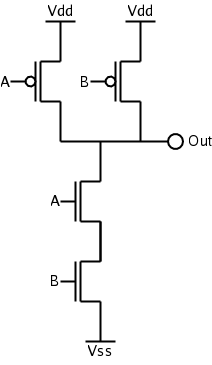
\includegraphics[width=0.5\textwidth]{media/ImplementationGates/CMOS_NAND.png}
\caption{Porte NON-ET avec des transistors MOSFET (Source : Wikimedia)}
\label{fig:NON-ET_MOS}
\end{figure}

\begin{figure}
\centering
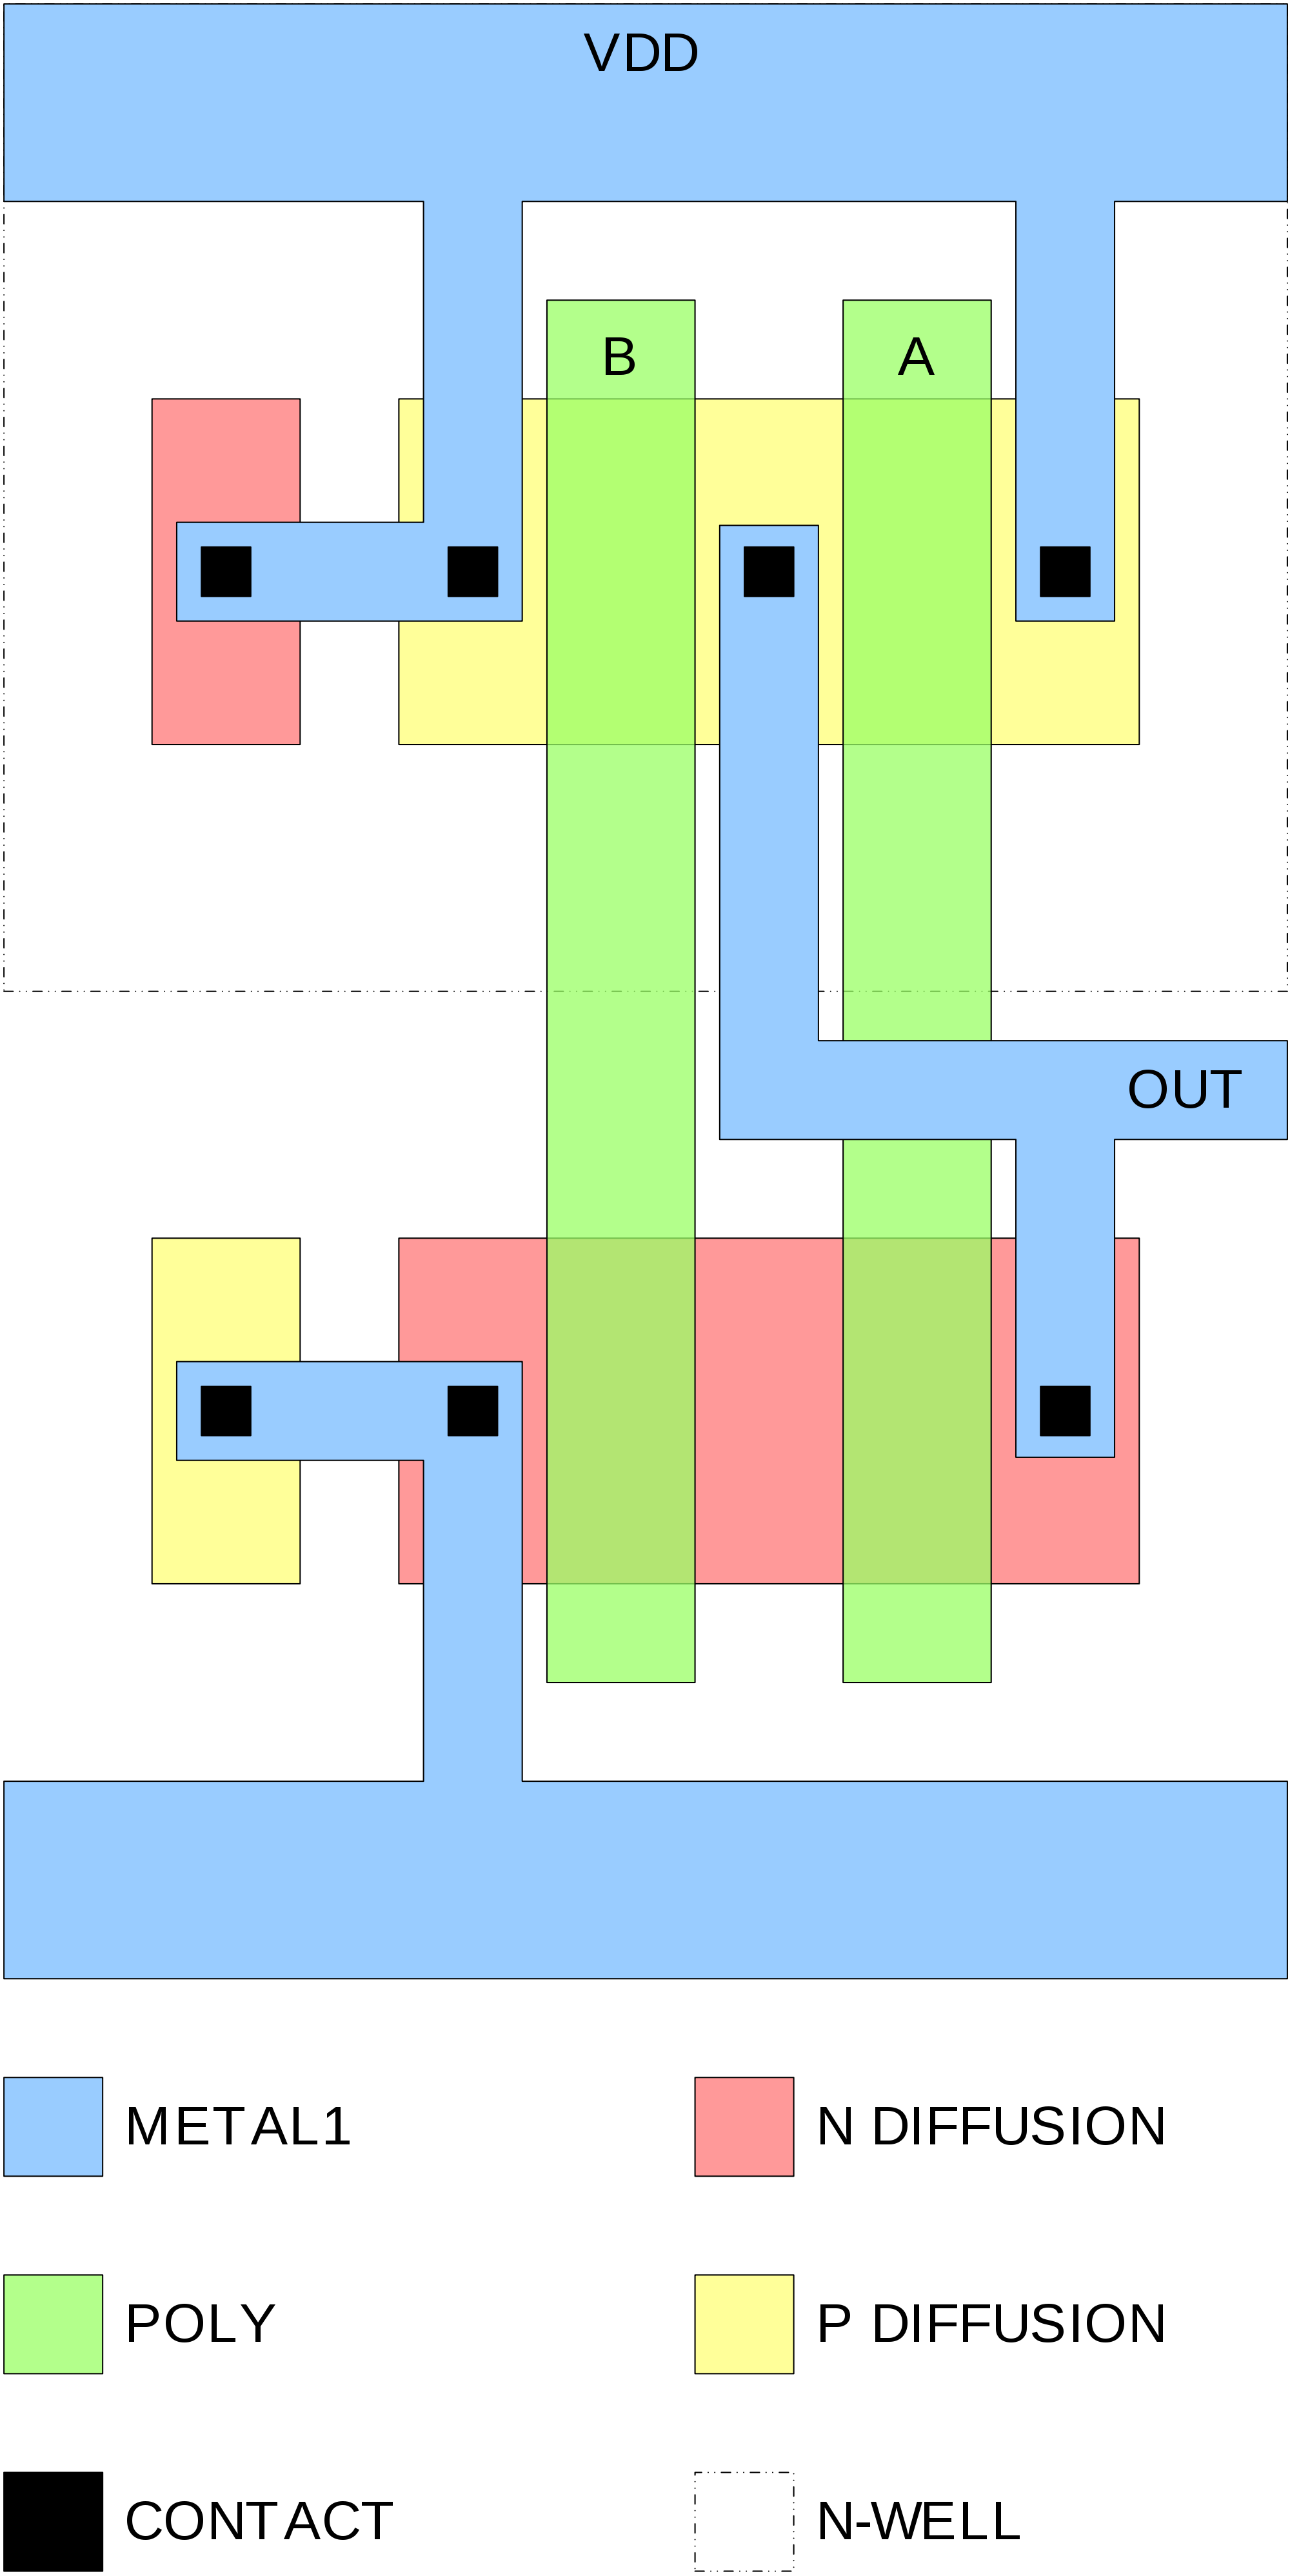
\includegraphics[width=0.5\textwidth]{media/ImplementationGates/2000px-CMOS_NAND_Layout.svg.png}
\caption{Masques du circuit CMOS NON-ET (Source : Wikimedia)}
\label{fig:NON-ET_CMOS_MASK}
\end{figure}

\subsection{Portes OU et OU exclusif (XOR)}
De la même manière, on peut proposer une implémentation pour la poste OU (figure \ref{fig:OU_MOS}) et la poste OU exclusif (figure \ref{fig:XOR_MOS}).

\begin{figure}
\centering
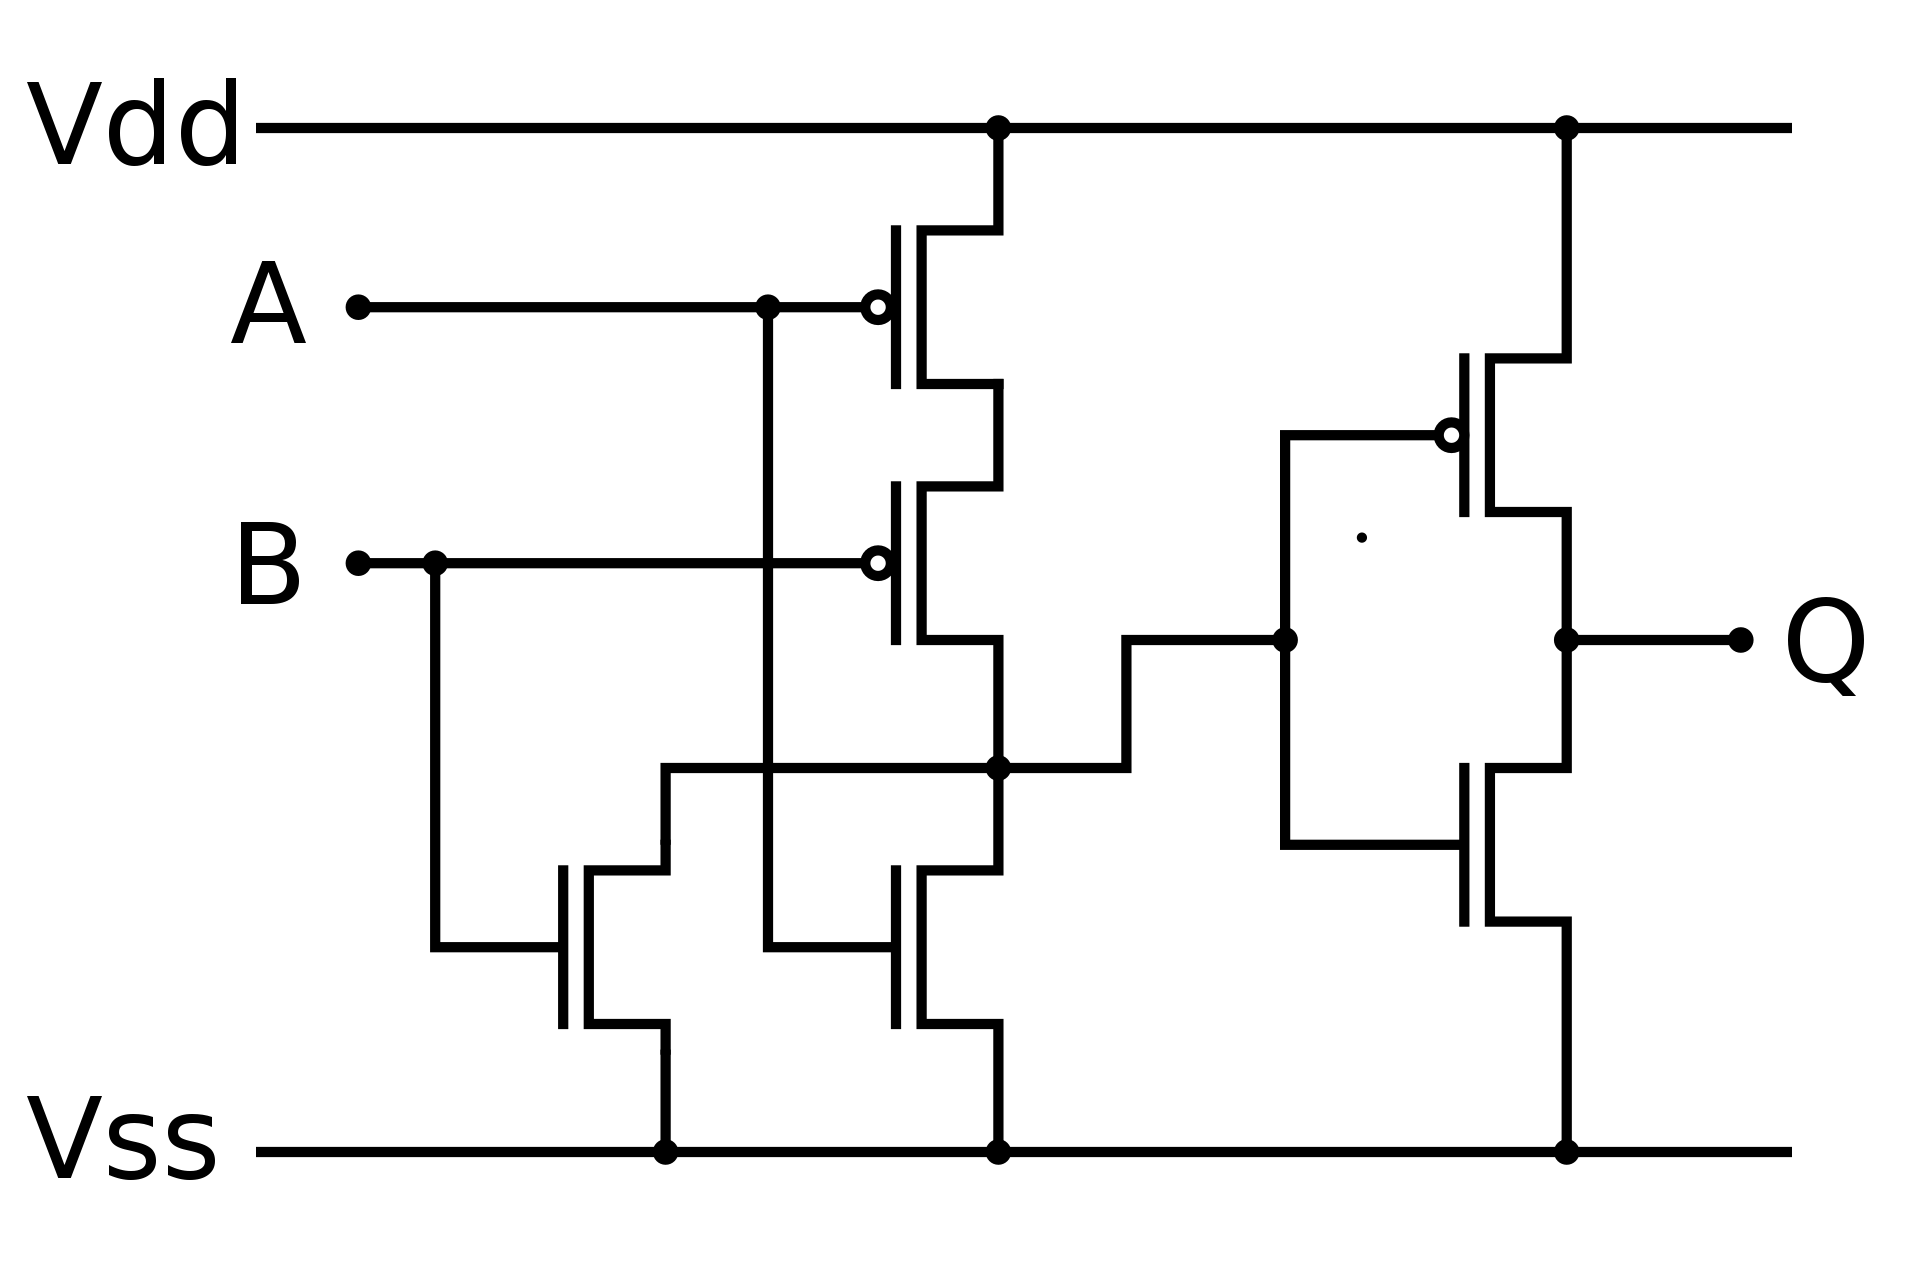
\includegraphics[width=0.5\textwidth]{media/ImplementationGates/1920px-CMOS_OR.svg.png}
\caption{Porte OU avec des transistors MOSFET (Source : Wikimedia)}
\label{fig:OU_MOS}
\end{figure}

\begin{figure}
\centering
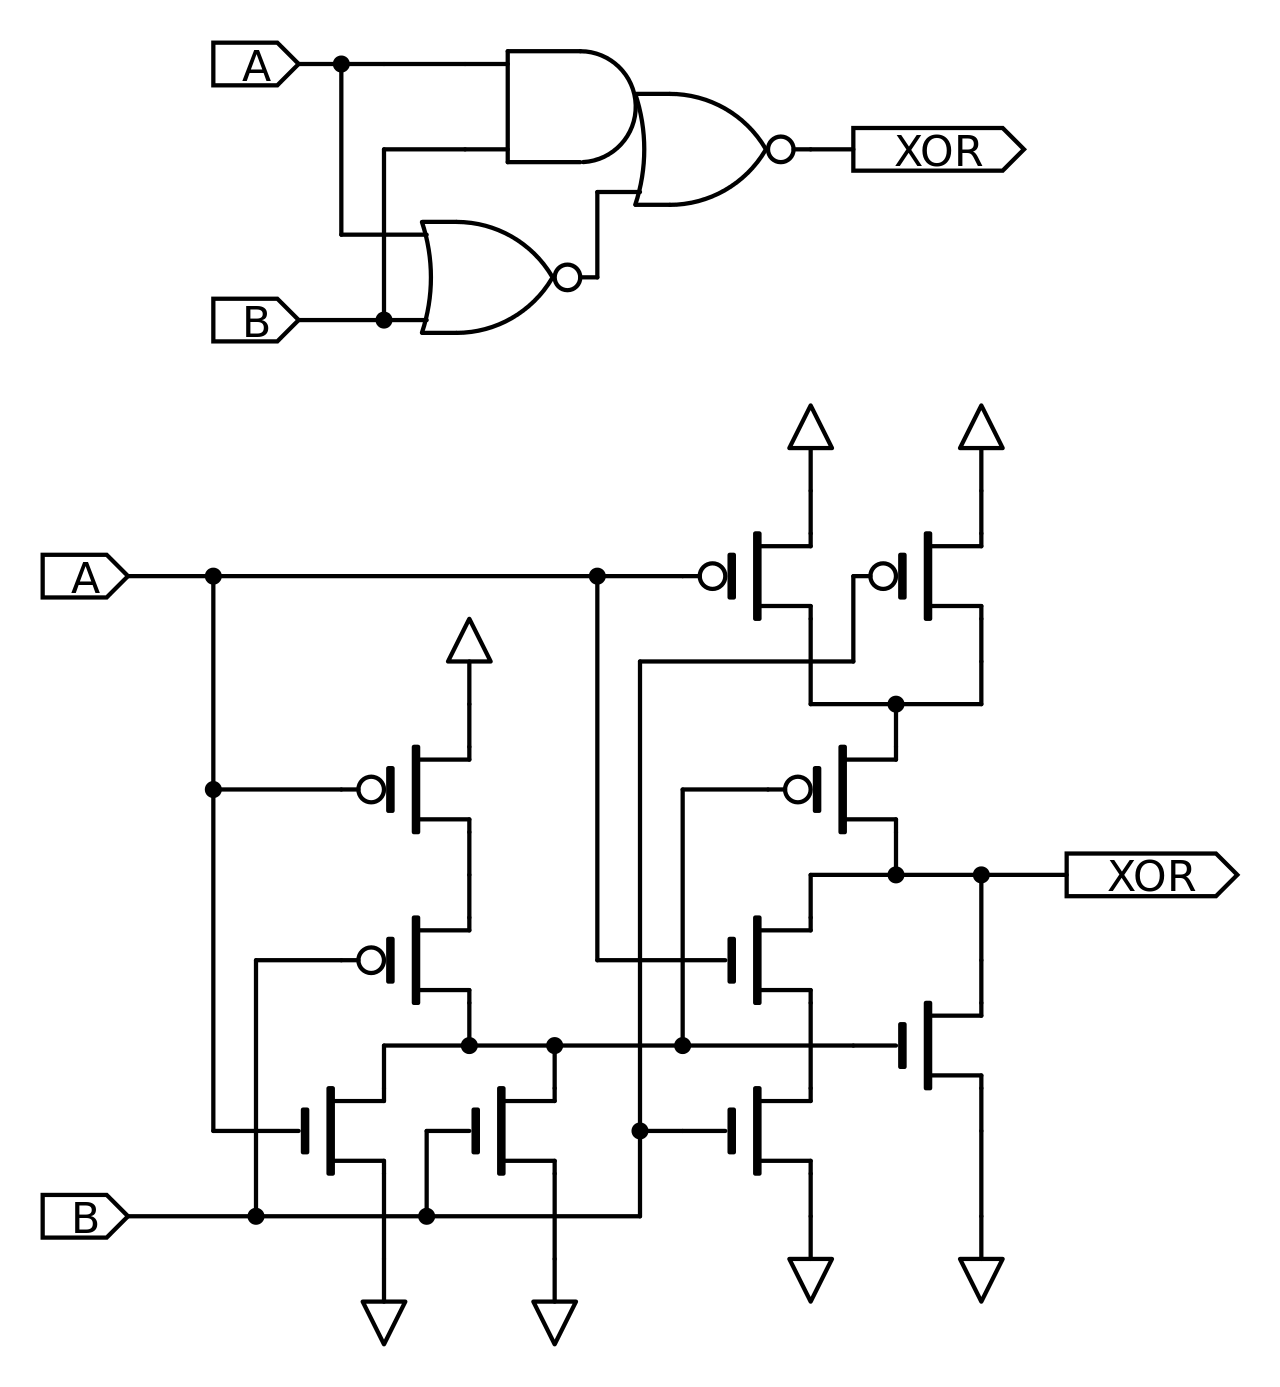
\includegraphics[width=0.5\textwidth]{media/ImplementationGates/1280px-CMOS10TrXOR.svg.png}
\caption{Portes XOR avec des transistors MOSFET (Source : Wikimedia)}
\label{fig:XOR_MOS}
\end{figure}

\end{document}